% !TEX TS-program = pdflatex
% !TEX encoding = UTF-8 Unicode

\documentclass[11pt]{article} % use larger type; default would be 10pt

\usepackage{pgf}
\usepackage{tikz}
\usetikzlibrary{arrows,automata,shapes}
\usetikzlibrary{decorations.pathmorphing} % LATEX and plain TEX when using Tik Z

\usepackage[utf8]{inputenc} % set input encoding (not needed with XeLaTeX)

%%% PAGE DIMENSIONS
\usepackage{geometry} % to change the page dimensions
\geometry{a4paper} % or letterpaper (US) or a5paper or....
\geometry{margin=2cm} % for example, change the margins to 2 inches all round
% \geometry{landscape} % set up the page for landscape
%   read geometry.pdf for detailed page layout information

\usepackage{graphicx} % support the \includegraphics command and options
\usepackage{subcaption} % for subfigures

\usepackage{scrextend} % https://tex.stackexchange.com/questions/588/how-can-i-change-the-margins-for-only-part-of-the-text
\usepackage{color}
\definecolor{rowcolor}{rgb}{0.94, 0.97, 1.0}  % 1=weiß, 0=schwarz

% \usepackage[parfill]{parskip} % Activate to begin paragraphs with an empty line rather than an indent

%%% PACKAGES
\usepackage{booktabs} % for much better looking tables
\usepackage{array} % for better arrays (eg matrices) in maths
\usepackage{paralist} % very flexible & customisable lists (eg. enumerate/itemize, etc.)
\usepackage{verbatim} % adds environment for commenting out blocks of text & for better verbatim
%\usepackage{subfig} % make it possible to include more than one captioned figure/table in a single float
% These packages are all incorporated in the memoir class to one degree or another...
\usepackage{listings} % Absatz als Code formatieren
\usepackage{floatflt} % für floatingfigure

%%% HEADERS & FOOTERS
\usepackage{fancyhdr} % This should be set AFTER setting up the page geometry
\pagestyle{fancy} % options: empty , plain , fancy
\renewcommand{\headrulewidth}{0pt} % customise the layout...
\lhead{ZIMFLI QCoDeS Driver}\chead{}\rhead{\today}
\lfoot{Michael Wagener}\cfoot{\thepage}\rfoot{FZJ/ZEA-2}

%%% SECTION TITLE APPEARANCE
\usepackage{sectsty}
\allsectionsfont{\sffamily\mdseries\upshape} % (See the fntguide.pdf for font help)
% (This matches ConTeXt defaults)

%%% ToC (table of contents) APPEARANCE
\usepackage[nottoc,notlof,notlot]{tocbibind} % Put the bibliography in the ToC
\usepackage[titles,subfigure]{tocloft} % Alter the style of the Table of Contents
\renewcommand{\cftsecfont}{\rmfamily\mdseries\upshape}
\renewcommand{\cftsecpagefont}{\rmfamily\mdseries\upshape} % No bold!

\usepackage{longtable} % Tabellen über mehrere Seiten
\usepackage{multirow} % multirow/multicolumn
\usepackage{colortbl} % farbige Tabellenzellen
\setlength{\LTpre}{0pt}  % Remove whitespace befor and after longtables
\setlength{\LTpost}{0pt}

\setlength{\tabcolsep}{1mm} % Setzt den Längenwert von {Abstand zwischen den Spalten einer Tabelle} auf den Wert 1mm
\setcounter{tocdepth}{2}  % Tiefe des Inhaltsverzeichnisses

\setlength{\parindent}{0em} % Damit die neuen Absätze nicht eingerückt werden

%%% END Article customizations

%%% The "real" document content comes below...

\title{QCoDeS driver for the Zurich Instruments Lock-In Amplifier (ZIMFLI)}
\author{Michael Wagener}

\begin{document}
\maketitle

\tableofcontents % toc anzeigen

\ \\
%\ \\

\begin{longtable}{|p{2.7cm}|p{2.6cm}|p{10.3cm}|}
\caption{Document revision history} \\
\hline\rowcolor{rowcolor}{\bf Date} & {\bf Author} & {\bf Short description} \\
\endfirsthead
\hline
08. Mar. 2019 & M.Wagener & First edit phase. \\ \hline
14. Mar. 2019 & M.Wagener & Complete the descriptions. \\ \hline
 &  &  \\ \hline
\end{longtable}


\clearpage

%%%
\section{Informations}

The Zurich Instruments Lock-In Amplifier (later only ZIMFLI) will be used in the QCoDeS Framework. Therefore a driver within this framework is needed.
My work was to implement / extend the first driver version and to test it and write a user documentation (this file). \\[0.5em]
%
All tests are done with the ZIMFLI with the serial number 4039 in the ZEA-2. This device has the F5M option installed (means 5MHz insteand of 500kHz frequency range). This device was registered in our LAN during my tests. \\[0.5em]
%
I use the Spyder environment with Python 3.6.

\subsection{Git and directories}

This driver is inside the QCoDeS framework tree under {\bf Qcodes/qcodes/instrument\_drivers/ZI}. In the subdirectory {\bf TestScripts} are my scripts with all my tests. They will be described later in this document. In the subdirectory {\bf Documentation} this documentation is located. The base of the QCoDeS framework I use during my tests is the git branch \\
\centerline{\it https://github.com/qutech/Qcodes/tree/feature/qctoolkit-integration}
This driver is pushed to the git branch \\
\centerline{\it https://github.com/qutech/Qcodes/tree/feature/ziMFLI\_driver}


\subsection{Additional installations needed}

\begin{floatingfigure}[r]{0.42\textwidth}
\mbox{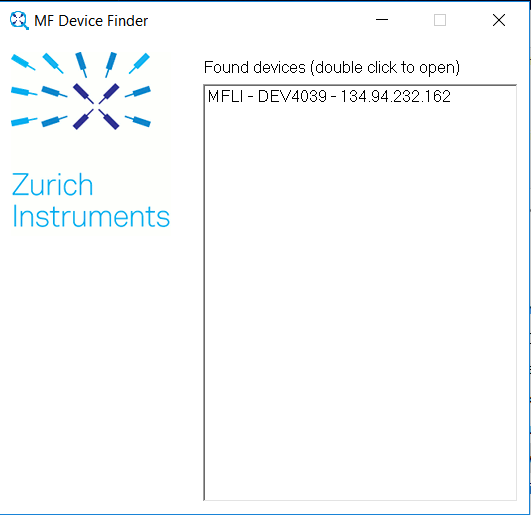
\includegraphics[width=0.4\textwidth]{ZI-DeviceFinder.png}}
\caption{ZI Device Finder}
\end{floatingfigure}
Don't forget to install the base driver from Zurich Instruments {\it https://www.zhinst.com/downloads}. Select the instrument {\it ``MFLI, MFIA''} and then the Software release version. Normally it is the best to leave the current version (for me it was 18.12). My first tests are done with the version 18.05 because the instrument has this version in its firmware. But the device runs also with the library-version 18.12. \\
Download and install the {\it Device Finder} for your Windows version or install the full packet {\it LabOne} for Windows or Linux. If you install the full packet, the documentation from ZI will also be installed.

You can connect the device to your USB port, the ZI software can install a special network driver for USB ports. After you connect the device to your network (or to your USB port), start the Device Finder and note the found device id.

Be sure that your computer is in the same subnet as the device. The device finder and later the driver cannot find the device if you use a VPN connection.

Then you have to install the Python package. From version 18.12 onwards you can start a shell and use the command
\begin{lstlisting}[frame=single]
pip install zhinst
\end{lstlisting}
All versions before have a separate download file on the ZI download page.

\clearpage


%%%
\section{General usage}

To use this driver, you have to import it and open the device. Be sure that you have the correct device id, it contains the serial number found with the {\it Device Finder}:

\begin{lstlisting}[frame=single, language=Python]
from qcodes.instrument_drivers.ZI.ZIMFLI import ZIMFLI
zidev = ZIMFLI( name='ZIMFLI', device_ID='DEV4039' )
\end{lstlisting}

During this open, the software searches for the device in the same subnet (or the USB). This will not work via VPN. The output in my test environment is:
\begin{lstlisting}[frame=single, language=Python]
Discovered device `dev4039`: MFLI with options F5M.
Creating an API session for device `dev4039` on `134.94.232.162`, `8004`
 with apilevel `6`.
\end{lstlisting}

In all following examples the variable {\bf zidev} is used as a reference to the device instance.

\ \\

After this you can access the device as decribed in detail later. As a first test you can get all version informations:
\begin{lstlisting}[frame=single, language=Python]
> import json
> print( json.dumps( zidev.version(), indent=4) )
{
    "DevType": "MFLI",
    "Options": "F5M",
    "Serial": "4039",
    "DevTime": "02.01.1970 10:41:25.265187",
    "Owner": "",
    "FPGARev": 52856,
    "DevFWRev": 53700,
    "BoardRev1": "1.4.G",
    "Copyright": "(c) 2008-2018 Zurich Instruments AG",
    "Dataserver": "ziDataServer",
    "ZI_FWRev": 0,
    "ZIRevision": 54618,
    "Version": "18.05"
}
\end{lstlisting}


\clearpage

%%%
\section{Base parameters}

The following parameters are accessible directly from the main device instance.

\begin{itemize}
\item zidev.{\bf oscillator1\_freq}( {\it value} ) \\
	Reads (without a value) or writes the frequency of the oscillator. Before writing, the driver checks the valid range from 0 Hz to 500 kHz ( or 5 MHz if the F5M option is installed).
\item zidev.oscillator2\_freq( {\it value} ) \\
	Same for the second oscillator if the MD option is installed.
\item zidev.oscillator3\_freq( {\it value} ) \\
	Same for the third oscillator if the MD option is installed.
\item zidev.oscillator4\_freq( {\it value} ) \\
	Same for the fourth oscillator if the MD option is installed.

\item zidev.{\bf bufferedReader}( demod\_index, total\_time, dolog, copyFreq, copyPhase, copyDIO, copyTrigger, copyAuxin ) \\
	Read the sample informations from the given demodulator for a given time and returns it as a dict of arrays. The parameters are:
	\begin{longtable}{p{1.5cm}p{3cm}p{12cm}}
	&demod\_index & index of demodulator channel (1,2) \\
	&total\_time  & number of seconds for measurement, this time the function is blocking \\
	&dolog & Flag if this function print some informations during running (elapsed time and data length) \\
	&copyFreq & Flag to copy the frequency data \\
	&copyPhase & Flag to copy the phase data \\
	&copyDIO & Flag to copy the digital I/O data \\
	&copyTrigger & Flag to copy the trigger data \\
	&copyAuxin & Flag to copy both auxin port data \\
	& \multicolumn{2}{p{15cm}}{\it The copy flags can be set to False (default if omitted) to preserve memory usage. Set them to True to get more arrays in the resulting dict.} \\
	\end{longtable}
	\textbf{\textit{Return:}} a dict with dict\_keys(['timestamp', 'x', 'y', {\it 'frequency'}, {\it 'phase'}, {\it 'dio'}, {\it 'trigger'}, {\it 'auxin0'}, {\it 'auxin1'}, 'time', 'R', 'phi'])
	The fields `R' and `phi' are calculated from `x' and `y'. The italic fields can be switched off with the copy flags. The field 'time' has the values:
	\begin{itemize}[ ]
	\itemsep0pt
	\item 'trigger': 0
	\item 'dataloss': False,
	\item 'blockloss': False,
	\item 'ratechange': False,
	\item 'invalidtimestamp': False,
	\item 'mindelta': 0,
	\item 'clockbase': 60000000.0  {\it this is used to calculate the correct time from the timestamps}
  	\end{itemize}

\item zidev.{\bf version}() \\
  	Read all possible version informations and returns them as a dict. See the first example above.

\item zidev.{\bf getLastSampleTimestamp()} \\
	Get the time of last sample request. The return is a three value array:
	\begin{longtable}{p{1.5cm}p{0.5cm}p{14.4cm}}
	& [0] & the current system time in seconds from time.time(). \\
	& [1] & the timestamp value of the device. \\
	& [2] & the timestamp of the device divided by the clockbase to get seconds. The absolute value of the seconds is not relevant because there is no function to set the current time, but the differences are useful. \\
	\end{longtable}

\item zidev.{\bf Scope} \\
  	Submodule for the scope functionality. This is under development.
 	
\item zidev.{\bf getClockbase()} \\
	Value of the clockbase to calculate the correct time from the timestamps.
	%%% --> Beispiel ?

\item zidev.{\bf getOptions()} \\
	Option string from the device. This string is read at the start of the driver from the device to apply the correct parameters and values.
  
\end{itemize}


%%%
\section{Submodules}

In this section I describe all implemented submodules for this device. For each submodule all available parameters are described.

\subsection{Demodulator}
The Lock-In-Amplifier has two demodulator channels. Not all parameters are accessible for the second channel. If the MD option is installed, there are four channels available. The submodules are named {\bf demod1} and {\bf demod2}, \small{with the MD option up to demod4}. The class is {\it DemodulatorChannel} with the following parameters:
	\begin{itemize}
	\item {\bf bypass}: Allows to bypass the demodulator low-pass filter, thus increasing the bandwidth.
	\item {\bf frequency}: {\it (ReadOnly)} Indicates the frequency used for demodulation and for output generation. The demodulation frequency is calculated with oscillator frequency times the harmonic factor. When the MOD option is used, linear combinations of oscillator frequencies including the harmonic factors define the demodulation frequencies.
	\item {\bf order}: Selects the filter roll off. Allowed Values:
	\begin{longtable}{p{1.5cm}p{1cm}p{14cm}}
	& 1 & 1st order filter 6 dB/oct \\
	& 2 & 2nd order filter 12 dB/oct \\
	& 3 & 3rd order filter 18 dB/oct \\
	& 4 & 4th order filter 24 dB/oct \\
	& 5 & 5th order filter 30 dB/oct \\
	& 6 & 6th order filter 36 dB/oct \\
	& 7 & 7th order filter 42 dB/oct \\
	& 8 & 8th order filter 48 dB/oct \\
	\end{longtable}
	\item {\bf harmonic}: Multiplies the demodulator's reference frequency by an integer factor. If the demodulator is used as a phase detector in external reference mode (PLL), the effect is that the internal oscillator locks to the external frequency divided by the integer factor.
	\item {\bf oscselect}: Connects the demodulator with the supplied oscillator. Number of available oscillators depends on the installed options. Is a number between 0 and the number of oscillators -1.
	\item {\bf phaseadjust}: Adjust the demodulator phase automatically in order to read 0 degrees.
	\item {\bf phaseshift}: Phase shift applied to the reference input of the demodulator. The value is clipped by the device to -180 .. +180 degrees.
	\item {\bf timeconstant}: Sets the integration time constant or in other words, the cutoff frequency of the demodulator low pass filter.
	\item {\bf samplerate}$^{(*)}$: Defines the demodulator sampling rate, the number of samples that are sent to the host computer per second. A rate of about 7-10 higher as compared to the filter bandwidth usually provides sufficient aliasing suppression. This is also the rate of data received by LabOne Data Server and saved to the computer hard disk. This setting has no impact on the sample rate on the auxiliary outputs connectors. Note: the value inserted by the user may be approximated to the nearest value supported by the instrument.
	\item {\bf sample}$^{(*)}$: {\it (ReadOnly)} Returns a dict with streamed demodulator samples with sample interval defined by the demodulator data rate. See note below. The dict contains the following entries:
	\begin{longtable}{p{1.5cm}p{3cm}p{12cm}}
	& 'timestamp' & array of uint64 with the internal timestamp of the measurement. Divide this by zidev.clockbase to get the real time in seconds. \\
	& 'x' & array of double with the x part of the demodulated cartesian coordinates \\
	& 'y' & array of double with the y part of the demodulated cartesian coordinates \\
	& 'frequency' & array of double with the current frequency of the oscillator \\
	& 'phase' & array of double with the angle of the demodulator polar coordinates \\
	& 'dio' & array of uint32 with the values of the digital inputs \\
	& 'trigger' & array of uint32 \\
	& 'auxin0' & array of double with the voltage of the first auxiliary input \\
	& 'auxin1' & array of double with the voltage of the second auxiliary input \\
	& 'R' & array of double with the calculated radius of the demodulated polar coordinates, see note below. \\
	& 'phi' & array of double with the calculated angle of the demodulated polar coordinates, see note below. \\
	\end{longtable}
	\item {\bf sinc}: Enables the sinc filter. When the filter bandwidth is comparable to or larger than the demodulation frequency, the demodulator output may contain frequency components at the frequency of demodulation and its higher harmonics. The sinc is an additional filter that attenuates these unwanted components in the demodulator output. Possible values are: `ON', `OFF'.
	\item {\bf signalinput}: Selects the input signal for the demodulator. Possible values: 'Sig In 1', 'Curr In 1', 'Trigger 1', 'Trigger 2', 'Aux Out 1', 'Aux Out 2', 'Aux Out 3', 'Aux Out 4', 'Aux In 1', 'Aux In 2', 'Constant input'.
	\item {\bf streaming}$^{(*)}$: Enables the data acquisition for the corresponding demodulator. Possible values are: `ON', `OFF'.
	\item {\bf trigger}$^{(*)}$: Selects the acquisition mode (i.e. triggering) or the demodulator. The possible values are:
	\begin{longtable}{p{0.8cm}p{3.1cm}p{12.6cm}}
	&'Continuous' & demodulator data is continuously streamed to the host computer \\
	&'Trigger in 1 Rise' & rising edge triggered \\
	&'Trigger in 1 Fall' & falling edge triggered \\
	&'Trigger in 1 Both' & triggering on both rising and falling edge \\
	&'Trigger in 2 Rise' & rising edge triggered \\
	&'Trigger in 2 Fall' & falling edge triggered \\
	&'Trigger in 2 Both' & triggering on both rising and falling edge \\
	&'Trigger in 1$\mid$2 Rise' & rising edge triggered on either input \\
	&'Trigger in 1$\mid$2 Fall' & falling edge triggered on either input \\
	&'Trigger in 1$\mid$2 Both' & triggering on both rising and falling edge or either trigger input \\
	&'Trigger in 1 Low' & demodulator data is streamed to the host computer when the level is low (TTL) \\
	&'Trigger in 1 High' & demodulator data is streamed to the host computer when the level is high (TTL) \\
	&'Trigger in 2 Low' & demodulator data is streamed to the host computer when the level is low (TTL) \\
	&'Trigger in 2 High' & demodulator data is streamed to the host computer when the level is high (TTL) \\
	&'Trigger in 1$\mid$2 Low' & demodulator data is streamed to the host computer when either level is low (TTL) \\
	&'Trigger in 1$\mid$2 High' & demodulator data is streamed to the host computer when either level is high (TTL) \\
	\end{longtable}
	\item {\bf x}: {\it (ReadOnly)} get sample of x coordinate. See note below.
	\item {\bf y}: {\it (ReadOnly)} get sample of y coordinate. See note below.
	\item {\bf R}: {\it (ReadOnly)} get sample of absolute value of x+y*i. See note below.
	\item {\bf phi}: {\it (ReadOnly)} get sample of angle of x+y*i. See note below.
	\item {\bf cfgTimeout}: stores the  used timeout in seconds for the readings of sample data (default 0.07). The valid range is from 0 to 1 second.
	\item $^{(*)}$ all parameters marked with this are only accessible for channel 1 or if the MD option is installed on other channels.
	\end{itemize}
	{\bf Note:} {\it The values of x and y are inside the sample dict, the values of R and phi are calculated. To have all values at the same measurement timestamp, the driver asks the device only if the last sample request is more than the cfgTimeout seconds ago.}


\subsection{Signal Input (Voltage)}
The Lock-In-Amplifier has one voltage sensitive input channel. The submodule is named {\bf signal\_in1}, the class is {\it SignalInputChannel} with the following parameters:
\begin{itemize}
\item {\bf autorange}: Automatic adjustment of the Range to about two times the maximum signal input amplitude measured over about 100 ms.
\item {\bf range}: Defines the gain of the analog input amplifier. The range should exceed the incoming signal by roughly a factor two including a potential DC offset. The instrument selects the next higher available range relative to a value inserted by the user. A suitable choice of this setting optimizes the accuracy and signal-to-noise ratio by ensuring that the full dynamic range of the input ADC is used.
\item {\bf float}: Switches the input between floating (ON) and connected to ground (OFF). This setting applies both to the voltage and the current input. It is recommended to discharge the test device before connecting or to enable this setting only after the signal source has been connected to the Signal Input in grounded mode.
\item {\bf scaling}: Applies the given scaling factor to the input signal.
\item {\bf ac}: Defines the input coupling for the Signal Inputs. AC coupling inserts a high-pass filter. OFF means DC ccoupling.
\item {\bf impedance}: Switches between 50 Ohm (ON) and 10 M Ohm (OFF).
\item {\bf diff}: Switches between single ended (OFF, use only +V input) and differential (ON, use both +V and -V inputs) measurements.
\item {\bf max}: Indicates the maximum measured value at the input.
\item {\bf min}: Indicates the minimum measured value at the input.
\item {\bf on}: Enables the signal input.
\item {\bf trigger}: Switches to the next appropriate input range such that the range fits best with the measured input signal amplitude.
\end{itemize}


\subsection{Signal Input (Current)}
The device has one current sensitive input channel. The submodule is named {\bf current\_in1}, the class is {\it CurrentInputChannel} with the following parameters:
\begin{itemize}
\item {\bf autorange}: Automatic adjustment of the Range to about two times the maximum signal input amplitude measured over about 100 ms.
\item {\bf range}: Defines the gain of the analog input amplifier. The range should exceed the incoming signal by roughly a factor two including a potential DC offset. The instrument selects the next higher available range relative to a value inserted by the user. A suitable choice of this setting optimizes the accuracy and signal-to-noise ratio by ensuring that the full dynamic range of the input ADC is used.
\item {\bf float}: Switches the input between floating (ON) and connected to ground (OFF). This setting applies both to the voltage and the current input. It is recommended to discharge the test device before connecting or to enable this setting only after the signal source has been connected to the Signal Input in grounded mode.
\item {\bf scaling}: Applies the given scaling factor to the input signal.
\item {\bf max}: Indicates the maximum measured value at the input.
\item {\bf min}: Indicates the minimum measured value at the input.
\item {\bf on}: Enables the signal input.
\item {\bf trigger}: Switches to the next appropriate input range such that the range fits best with the measured input signal amplitude.
\end{itemize}


\subsection{Auxiliary Inputs}
The device has two auxiliary inputs. Because of the demodulator functionality the input values are only available as fields in the dict of the demodulator sample reading. The submodule is named {\bf aux\_in1}, the class is {\it AUXInputChannel} with the following parameters:
\begin{itemize}
\item {\bf averaging}: Defines the number of samples on the input to average as a power of two. Possible values are in the range [0, 16]. A value of 0 corresponds to the sampling rate of the auxiliary input's ADC.
\item {\bf sample}: This returns the same dict as the demodulator parameter sample.
\end{itemize}


\subsection{External reference}
The device has the capability to synchronize its internal oscillator used for demodulation with an external reference clock signal. The submodule is named {\bf extref1}, the class is {\bf ExternalReferenceChannel} with the following parameters:
\begin{itemize}
\item {\bf signalin}: {\it (ReadOnly)} Indicates the input signal selection for the selected demodulator. Possible Values are 'Sig In 1', 'Curr In 1', `Trigger 1', 'Trigger 2', 'Aux Out 1', 'Aux Out 2', 'Aux Out 3', 'Aux Out 4', 'Aux In 1', 'Aux In 2', `Constant'.
\item {\bf automode}: {\it (Only with MD option installed)} This defines the type of automatic adaptation of parameters in the PID used for external reference. Allowed values are 'None', 'PID Auto', 'PID Low', 'PID High', 'PID All'.
\item {\bf bandwidth}: {\it (Only without MD option installed)} This defines the bandwidth used for external reference. Allowed values are `None', `Low', `High'.
\item {\bf channel}: {\it (ReadOnly)} Indicates the demodulator connected to the extref channel.
\item {\bf enable}: Enables the external reference. Allowed Values are `ON' and `OFF'.
\item {\bf locked}: {\it (ReadOnly)} Indicates whether the external reference is locked.
\item {\bf oscselect}: {\it (ReadOnly)} Indicates which oscillator is being locked to the external reference.
\end{itemize}
In the following example the external reference is switched on, set to low bandwidth and the input is set to the auxiliary input 1:
% die Leerzeichen vor den # sind abgezählt damit die # übereinander stehen!
\begin{lstlisting}[frame=single, language=Python]
er = zidev.submodules['extref1']  # select submodule
er.enable('ON')                   # switch external reference on
er.bandwidth('Low')               # select low bandwidth
dm2 = zidev.submodules['demod2']  # get another submodule
dm2.signalin('Aux In 1')          # select input for external reference
\end{lstlisting}


\subsection{Signal Output}
The device has one signal output. The submodule is named {\bf signal\_out1}, the class is {\it SignalOutputChannel} with the following parameters:
\begin{itemize}
\item {\bf add}: The signal supplied to the Aux Input 1 is added to the signal output. For differential output the added signal is a common mode offset. The allowed values are `ON' and `OFF'.
\item {\bf autorange}: If enabled, selects the most suited output range automatically. Allowed values are `ON' and `OFF'.
\item {\bf differential}: Switch between single-ended output (OFF) and differential output (ON). In differential mode the signal swing is defined between Signal Output +V and -V.
\item {\bf imp50}: Select the load impedance between 50 Ohm (ON) and HiZ (OFF). The impedance of the output is always 50 Ohm. For a load impedance of 50 Ohm the displayed voltage is half the output voltage to reflect the voltage seen at the load.
\item {\bf offset}: Defines the DC voltage that is added to the dynamic part of the output signal. Currently this value is only valid for the driver in the range from -1.5V to +1.5V.
\item {\bf on}: Enabling/Disabling the Signal Output. Corresponds to the blue LED indicator on the instrument front panel.
\item {\bf overloaded}: {\it (ReadOnly)} Indicates that the signal output is overloaded.
\item {\bf range}: Sets the output voltage range. Currently this value is only valid for the driver in the range from 0.001 to 3.0. The device will select the next higher available range automatically.
\item {\bf amplitude}: Sets the peak amplitude that the oscillator assigned to the given demodulation channel contributes to the signal output. Should be given as Vpk value.
\item {\bf ampdef}: Internal storage for the used unit for the amplitude. Possibla values are `Vpk', `Vrms' or `dBm', default is `Vpk'.
\item {\bf enable}: Enables individual output signal amplitude. {\it When the MD option is installed, it is possible to generate signals being the linear combination of the available demodulator frequencies.}
\end{itemize}


\subsection{Auxilliary Outputs}
The device has four auxiliary outputs. The submodules are named {\bf aux\_out1} .. {\bf aux\_out4}, the class is {\it AUXOutputChannel} and has the following parameters:
\begin{itemize}
\item {\bf scale}: Multiplication factor to scale the signal.
\item {\bf preoffset}: Add a pre-offset to the signal before scaling is applied.
\item {\bf offset}: Add the specified offset voltage to the signal after scaling.
\item {\bf limitlower}: Lower limit for the signal at the Auxiliary Output. A smaller value will be clipped. Can have a value between -10 an 10 V.
\item {\bf limitupper}: Upper limit for the signal at the Auxiliary Output. A larger value will be clipped. Can have a value between -10 an 10 V.
\item {\bf channel}: channel according to the selected signal source
\item {\bf output}: signal source of the signal to amplify. Allowed values are 'Demod X', 'Demod Y', 'Demod R', 'Demod THETA', 'PID Out', 'PID Shift', 'PID Error', 'TU Filtered Value', 'TU Output Value'
\item {\bf value}: {\it (ReadOnly)} Voltage present on the Auxiliary Output. \\
\centerline{Auxiliary Output Value = ( Signal + Preoffset ) * Scale + Offset}
\end{itemize}


\subsection{Trigger Inputs}
The Lock-In-Amplifier has two TTL compatible trigger input lines. The connectors are on the back side of the device. The submodules are named {\bf trigger\_in1} and {\bf trigger\_in2}, the class is {\it TriggerInputChannel} and has the following parameters:
\begin{itemize}
\item {\bf autothreshold}: Automatically adjust the trigger threshold. The level is adjusted to fall in the center of the applied transitions. Allowed values are `ON' and `OFF'.
\item {\bf level}: Trigger voltage level at which the trigger input toggles between low and high. Use 50\% amplitude for digital input and consider the trigger hysteresis.
\end{itemize}


\subsection{Trigger Outputs}
The Lock-In-Amplifier has two TTL compatible trigger output lines. The connectors are on the back side of the device. The submodules are named {\bf trigger\_out1} and {\bf trigger\_out2}, the class is {\it TriggerOutputChannel} and has the following parameters:
\begin{itemize}
\item {\bf pulsewidth}: Defines the minimal pulse width for the case of Scope events written to the trigger outputs of the device. Currently this value is only valid for the driver in the range from 0 to 0.149 seconds.
\item {\bf source}: Select the signal assigned to the trigger output. Possible values are:
	\begin{itemize}[ ]
	\itemsep0pt
	\item 'disabled'
	\item 'osc phase of demod 2' {\it (only without installed MD option)}
	\item 'osc phase of demod 4' {\it (only if MD option is installed)}
	\item 'Threshold Logic Unit 1'
	\item 'Threshold Logic Unit 2'
	\item 'Threshold Logic Unit 3'
	\item 'Threshold Logic Unit 4'
	\item 'MDS Sync Out'
  	\end{itemize}
\end{itemize}


\subsection{Digital Input / Outputs}
The Lock-In-Amplifier has 32 digital input / output lines. They are available at a special connector located at the back of the device. The submodule is named {\bf dio}, the class is {\it DIOChannel} with the following parameters:
\begin{itemize}
\item {\bf decimation}: Sets the decimation factor for DIO data streamed to the host computer.
\item {\bf direction}: The 32 bits are separated into 4 groups of 8 bit. Each 8 bit group can be set to input or output separatly. This bitmask gives the direction and a bit value of 1 means output, a bit value of 0 means input:

% Definition der Block-Styles für die folgenden Flußdiagramme
\tikzstyle{block2} = [rectangle, draw, fill=white, text centered, minimum height=1.5em]
\tikzstyle{line} = [draw, -latex']
\begin{tikzpicture}[trim left=-4.2cm,every text node part/.style={align=center}]
	\node[block2, fill=yellow!10, text width=2cm] (BITX) at (0,0) {...};
	\node[block2, fill=yellow!10, anchor=west, text width=0.6cm] (BIT3) at (BITX.east) {3};
	\node[block2, fill=yellow!10, anchor=west, text width=0.6cm] (BIT2) at (BIT3.east) {2};
	\node[block2, fill=yellow!10, anchor=west, text width=0.6cm] (BIT1) at (BIT2.east) {1};
	\node[block2, fill=yellow!10, anchor=west, text width=0.6cm] (BIT0) at (BIT1.east) {0};
	\node[anchor=east] at (BITX.west) {Bits of {\it direction}:};
	\node[anchor=north west, yshift=-0.1cm] (TXT0) at (BIT0.south) {for I/O 0 .. 7};
	\node[anchor=north west, yshift=-0.5cm] (TXT1) at (BIT1.south) {for I/O 8 .. 15};
	\node[anchor=north west, yshift=-0.9cm] (TXT2) at (BIT2.south) {for I/O 16 .. 23};
	\node[anchor=north west, yshift=-1.3cm] (TXT3) at (BIT3.south) {for I/O 24 .. 31};
	\draw [line, -] (BIT0.south) -- (TXT0.north west);
	\draw [line, <->] (BIT1.south) -- (TXT1.north west);
	\draw [line, <->] (BIT2.south) -- (TXT2.north west);
	\draw [line, <->] (BIT3.south) -- (TXT3.north west);
\end{tikzpicture}

\item {\bf extclk}: `OFF': internally clocked with a fixed frequency of 60 MHz, `ON':  externally clocked with a clock signal connected to DIO Pin 68. The available range is from 1 Hz up to the internal clock frequency
\item {\bf mode}: `Manual': Manual setting of the DIO output value. `Threshold unit': Enables setting of DIO output values by the threshold unit.
\item {\bf output}: Sets the value of the DIO output for those bytes where 'direction' is set to output.
\item The inputs are read in the sample dict of the demodulator.
\end{itemize}


\subsection{Multi device synchronization}
The feature Multi device synchronization can be used to sync more than one Lock.-In Amplifier to use always the same clock phase. For more informations please look into the manual. This feature is not tested. The submodule is named {\bf mds}, the class is {\it MDSChannel} with the following parameters:
\begin{itemize}
\item {\bf armed}: {\it (ReadOnly)} Indicates whether the mds module is armed and waiting for pulses.
\item {\bf drive}: Enables output of synch pulses on trigger output 1.
\item {\bf enable}: Enables the mds module.
\item {\bf source}: Select input source for mds synch signal.
\item {\bf syncvalid}: {\it (ReadOnly)} Indicates if sync pulses are received.
\item {\bf timestamp}: Used to set the resulting adjusted timestamp.
\end{itemize}


\subsection{Scope Channel}
        ** under development ***


\subsection{PID}
    Combines all parameters concerning the PIDs.
    These Parameters are only available if the MF-PID Quad PID/PLL Controller 
    option is installed on the MFLI parent Instrument.


\subsection{Sweeper}
The manual says that the sweeper option is only available if the MD option is installed (Multi Demodulator). In my test device this is not but the sweep function works in the Web-GUI. At the moment the driver disables all Sweeper functions.
% if "MD" in self.options:
%            self.sweeper = self.daq.sweep()
%            self.sweeper.set('sweep/device', self.device)
%class SweeperChannel(InstrumentChannel):
%    Combines all the parameters for the sweeper module.
%class Sweep(MultiParameter):
%    Parameter class for the ZIMFLI instrument class for the sweeper.
%    The get method returns a tuple of arrays, where each array contains the
%    values of a signal added to the sweep (e.g. demodulator 4 phase).


\end{document}
